
\chapter{License Compatibility Checking}
\label{ch:ch7}
\begin{flushright}
\textit{``What kind of Web do we want?’''} \\
 Tim Berners-Lee\footnote{\url{https://webwewant.org/}}
 \end{flushright}
 

\section*{Introduction}
\todo{add intro of what is about here} \\

\section{Background}
The license of a dataset in the Web of Data can be specified within the data, or outside of it, for example in a separate document linking the data. In line with the Web of Data philosophy~\cite{LinkedData2011}, licenses for such datasets should be specified in RDF, for instance through the Dublin Core vocabulary\footnote{\url{http://purl.org/dc/terms/license}}. Despite such guidelines, still a lot of effort is needed to enhance the association of licenses to data on the Web, and to process licensed material in an automated way. The scenario becomes even more complex when another essential component in the Web of Data is taken into account: the vocabularies. Our goal is to support the data provider in assigning a license to her data, and verifying its compatibility with the licenses associated to the adopted vocabularies.      


%
We answer this question by proposing an online framework called LIVE\footnote{The online tool is available at \url{http://www.eurecom.fr/~atemezin/licenseChecker/}} (LIcenses VErification) that exploits the formal approach to licenses composition proposed in~\cite{DBLP:conf/semweb/GovernatoriRVG13} to verify the compatibility of a set of heterogeneous licenses. LIVE, after retrieving the licenses associated to the vocabularies used in the dataset under analysis, supports data providers in verifying whether the license assigned to the dataset is compatible with those of the vocabularies, and returns a warning when this is not the case. 

\section{Statistics about licensed vocabularies}
\label{sec:stats-license}

The first step to be addressed consists in analyzing how many vocabularies are licensed, and what is the distribution of such licenses. To achieve this goal, we started our analysis on the Linked Open Vocabularies repository. The LOV initiative stands as an observatory for the re-usable linked vocabularies ecosystem. The initiative goes beyond collecting and highlighting vocabulary metadata, and it now plays a major social role in promoting good practice and improving overall ecosystem quality of publishing vocabularies\footnote{For more details about LOV, see \url{http://ercim-news.ercim.eu/en96/special/linked-open-vocabularies}}. We crawled the LOV repository together with the LODstats one searching for licensed vocabularies. The results we obtained are as follows:
\begin{description}
\item[Licensed vocabularies]: we have considered in total 419 vocabularies. The licensed vocabularies are 64 out of 419, eating about 16\% of the the total number of considered vocabularies. The properties used to specify the licenses in the vocabularies are \url{http://creativecommons.org/ns\#license} from the Creative Commons vocabulary~\footnote{\url{http://creativecommons.org/ns}} and \url{http://purl.org/dc/terms/license} from the Dublin Core vocabulary\footnote{\url{http://dublincore.org/documents/dcmi-terms/}}. Even if the number of licensed vocabularies available on LOV and LODstats is rather low, analyzing the edits of the licensing information it is possible to note an increasing interest in providing further metadata about the data published on the Web of Data, and it holds also for vocabularies\footnote{In this work, we consider vocabularies as data. Other interpretation of the role of vocabularies are discussed in the conclusions.}. Another interesting result shows that 4 out of 13 vocabularies retrieved searching for the ``top 20 most used entities in the LOD cloud\footnote{\url{http://lod-cloud.net/}}'' has an explicit license associated. These vocabularies are Good Relations\footnote{\url{http://purl.org/goodrelations/v1\#}}, DBpedia, GeoNames\footnote{\url{http://www.geonames.org/ontology\#}}, and FRBR\footnote{\url{http://vocab.org/frbr/core.html\#}}.   
\item[Licenses distribution]: the distribution of the licenses in the licensed vocabularies we retrieved is visualized in Figure~\ref{fig:LOVstats}. The most adopted license is Creative Commons Attribution (CC-BY) (30 out of 64 licensed vocabularies), and Creative Commons licenses in general represent the 85\% of the licenses used for vocabularies licensing, confirming the trend shown for licensed datasets~\cite{DBLP:conf/semweb/Rodriguez-DoncelGM13,DBLP:conf/semweb/GovernatoriRVG13}. Another popular license is ODC Public Domain Dedication and License (PDDL)\footnote{\url{http://opendatacommons.org/licenses/pddl/1.0/}} followed by the W3C Software Notice and License\footnote{\url{http://bit.ly/W3C-license}}.  
\end{description}

\begin{figure}
\centering
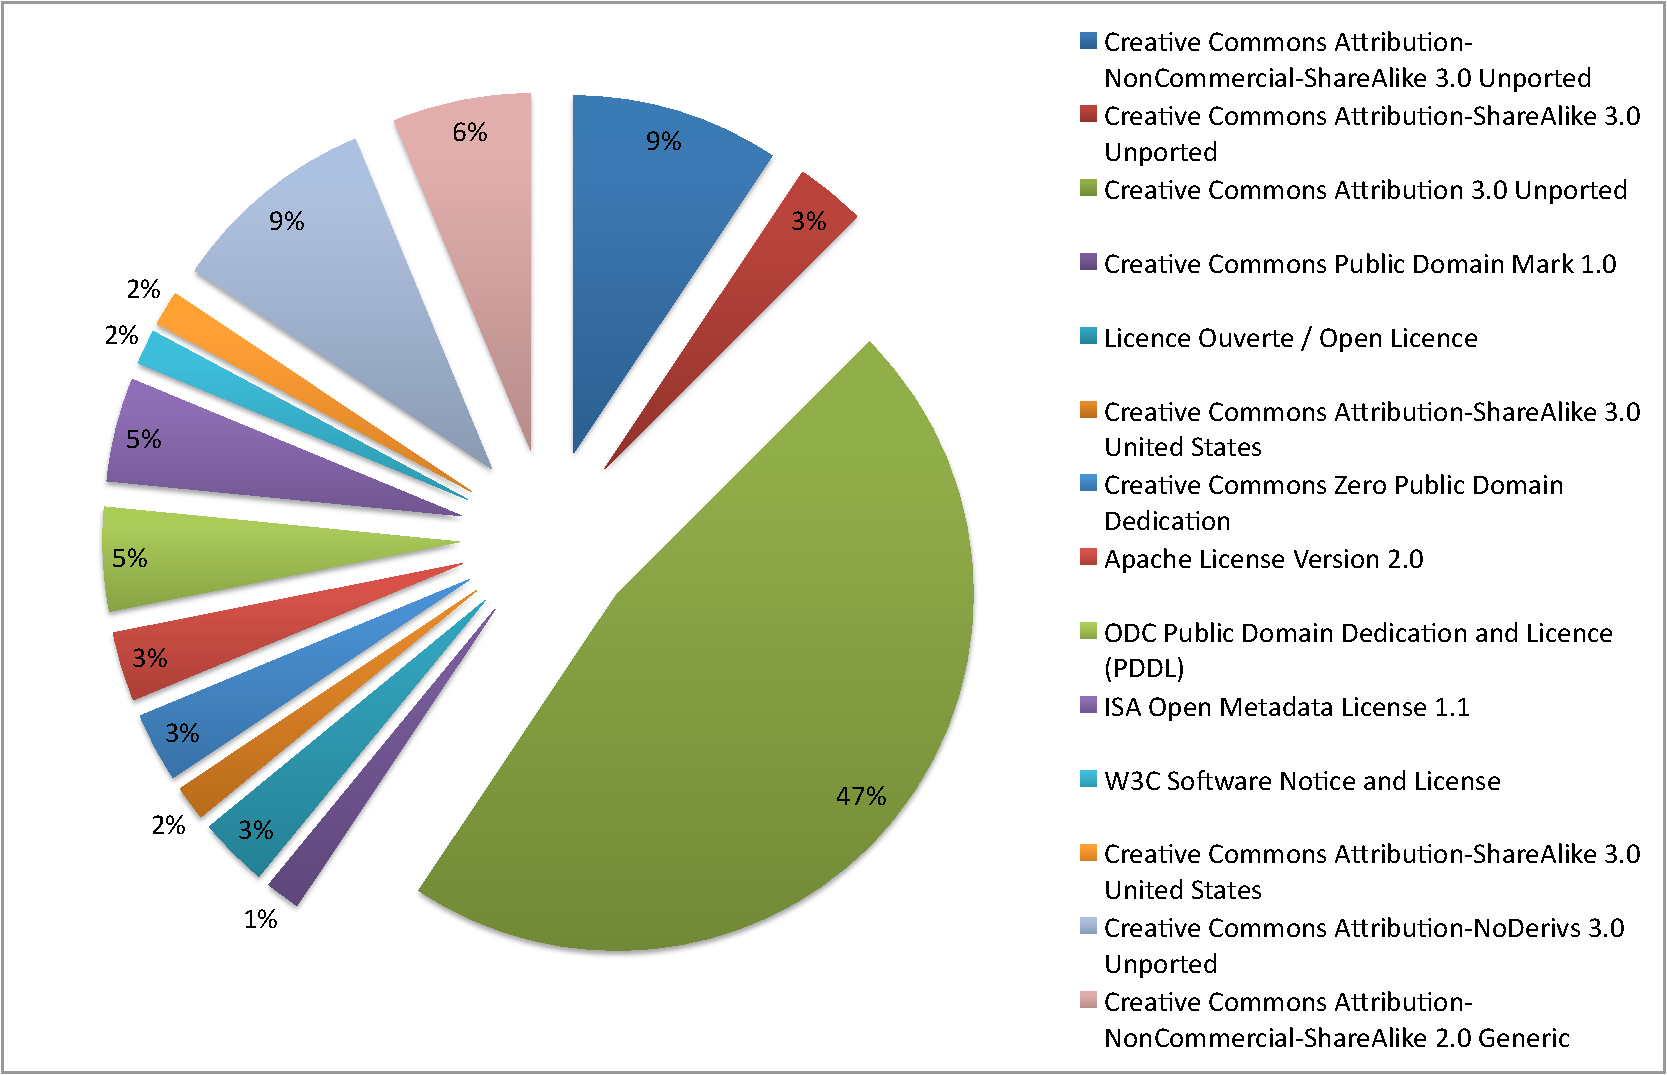
\includegraphics[width=9.5cm]{img/LOV-stats.pdf}
\caption{Licenses distribution in the LOV licensed vocabularies.}
\label{fig:LOVstats}
\end{figure}

We are aware that the obtained results are referred to the data available on LOV and LODstats, and that such repositories of vocabularies are not exhaustive. However, they provide us a reliable picture of what is the ongoing trend in licensing vocabularies\footnote{We refer the reader interested into statistics about the distribution of licenses on the Web of Data to~\cite{DBLP:conf/semweb/Rodriguez-DoncelGM13,DBLP:conf/semweb/GovernatoriRVG13}.}. This is particularly true in the case of LOV that furthermore supports a number of good practices for the publication of a vocabulary, among which the addition of the license associated to the vocabulary is highly encouraged.

\section{Related work about licenses in the Web of Data}

In the Web scenario, a number of works address the problem of representing and/or reasoning over licensing information.
Iannella~\footnote{\url{http://odrl.net/1.1/ODRL-11.pdf}} presents the Open Digital Rights Language (ODRL) for expressing rights information over content, and Gangadharan et al.~\cite{ODRLS} further extend ODRL developing the ODRL-S language to implement the clauses of service licensing. 
%
Gangadharan et al.~\cite{DBLP:conf/icsoc/GangadharanWDI07} address the issue of service license composition and compatibility analysis basing on ODRL-S. They specify a matchmaking algorithm which verifies whether two service licenses are compatible. In case of a positive answer, the services can be composed and the framework determines the license of the composite service. 
%
Nadah et al.~\cite{DBLP:conf/icail/NadahRB07} propose to assist licensors' work by providing them a generic way to instantiate licenses, independent from specific formats, and then they translate the license expressed in generic terms into more specific terms compliant with the specific standards used by distribution systems, i.e., ODRL and MPEG Rights Data Dictionaries. 
%
Truong et al.~\cite{DBLP:conf/apscc/TruongGCDP11} address the issue of analyzing data contracts, based on ODRL-S again. Contract analysis leads to the definition of a contract composition where first the comparable contractual terms from the different data contracts are retrieved, and second an evaluation of the new contractual terms for the data mash-up is addressed.
%
Krotzsch and Speiser~\cite{DBLP:conf/semweb/KrotzschS11} present a semantic framework for evaluating ShareAlike recursive statements. In particular, they develop a general policy modelling language, then instantiated with OWL DL and Datalog, for supporting self-referential policies as expressed by CC.
%
Gordon~\cite{DBLP:conf/icail/Gordon11} presents a legal prototype for analyzing open source licenses compatibility using the Carneades argumentation system. 
%
Finally, Rodiguez-Doncel et al.~\cite{victorPatterns2013a,victorPatterns2013b} discuss licenses patterns for Linked Data. In particular, they first analyze and discuss six rights expression languages, abstracting their commonalities and outlining their underlying pattern. Second, they propose the License Linked Data Resources pattern which provides a solution to describe existing licenses and rights expressions both for open and not open scenarios. 
All these works either propose new ways to model licenses information or new formal frameworks to deal with rights. In this paper, we do not address none of these issues, and we adopt the formal framework proposed in~\cite{DBLP:conf/semweb/GovernatoriRVG13}. Also Pucella and Weissman~\cite{DBLP:conf/csfw/PucellaW02} propose a logic to check whether the user's actions follow the licenses' specifications. However, as they do not deal with compatibility, do not provide a deontic account of licenses' conclusions, and their logic is not able to handle conflicting licenses, we choose and adapt the deontic logic of~\cite{DBLP:conf/semweb/GovernatoriRVG13}, which better suits our needs.

Up to our knowledge, the issue of licensed vocabularies has never been addressed. More precisely, no available framework exists dealing with such licenses and verifying in an automated way their potential compatibility with the license associated to datasets. The goal of supporting users in dealing with licensing information has been recently addressed by Cabrio et al.~\cite{CabrioESWC2014} with a different goal, i.e., supporting data publishers in creating RDF licenses representations from natural language texts. 

\section{The LIVE Framework}
\label{sec:live}
The LIVE framework is a Javascript application, combining HTML and Bootstrap. Hence, installation has no prerequisite. Since the tool is written in Javascript, the best way to monitor the execution time is with the \texttt{performance.now()} function. We use the $10$ LOD datasets with the highest number of links towards other LOD datasets available at \url{http://lod-cloud.net/state/#links}. For each of the URLs in Datahub, we retrieve the VoID\footnote{\url{http://www.w3.org/TR/void/}} file in Turtle format, and we use the \textit{voidChecker} function\footnote{\url{http://www.eurecom.fr/~atemezin/licenseChecker/voidChecker.html}} of the LIVE tool to retrieve the associated license, if any.  
The goal of the LIVE framework is to support data producers to assign a license to the data ensuring the consistency of such license with respect to the licenses assigned to the vocabularies she exploits in the dataset. 
The input of the LIVE framework (Figure~\ref{fig:framework}) consists in the dataset (URI or VOiD) whose license has to be verified. The framework is composed by two modules. The first module takes care of retrieving the vocabularies used in the dataset, and for each vocabulary, retrieves the associate license\footnote{Note that the LIVE framework relies on the dataset of machine-readable licenses (RDF, Turtle syntax) presented in~\cite{CabrioESWC2014}.} (if any) querying the LOV repository. 
The module searches out also the license associated to the dataset itself. When all the licensing information of interest has been obtained, the module provides such set of licenses to the compatibility checking module. 
The second module takes as input the set of licenses (i.e., the licenses of the vocabularies used in the dataset as well as the license assigned to the dataset) to verify whether they are compatible with each others. The result returned by the module is a \textit{yes/no} answer. In case of negative answer, the data provider is invited to change the license associated to the dataset and check back again with the LIVE framework whether further inconsistencies arise.

\begin{figure}
\centering
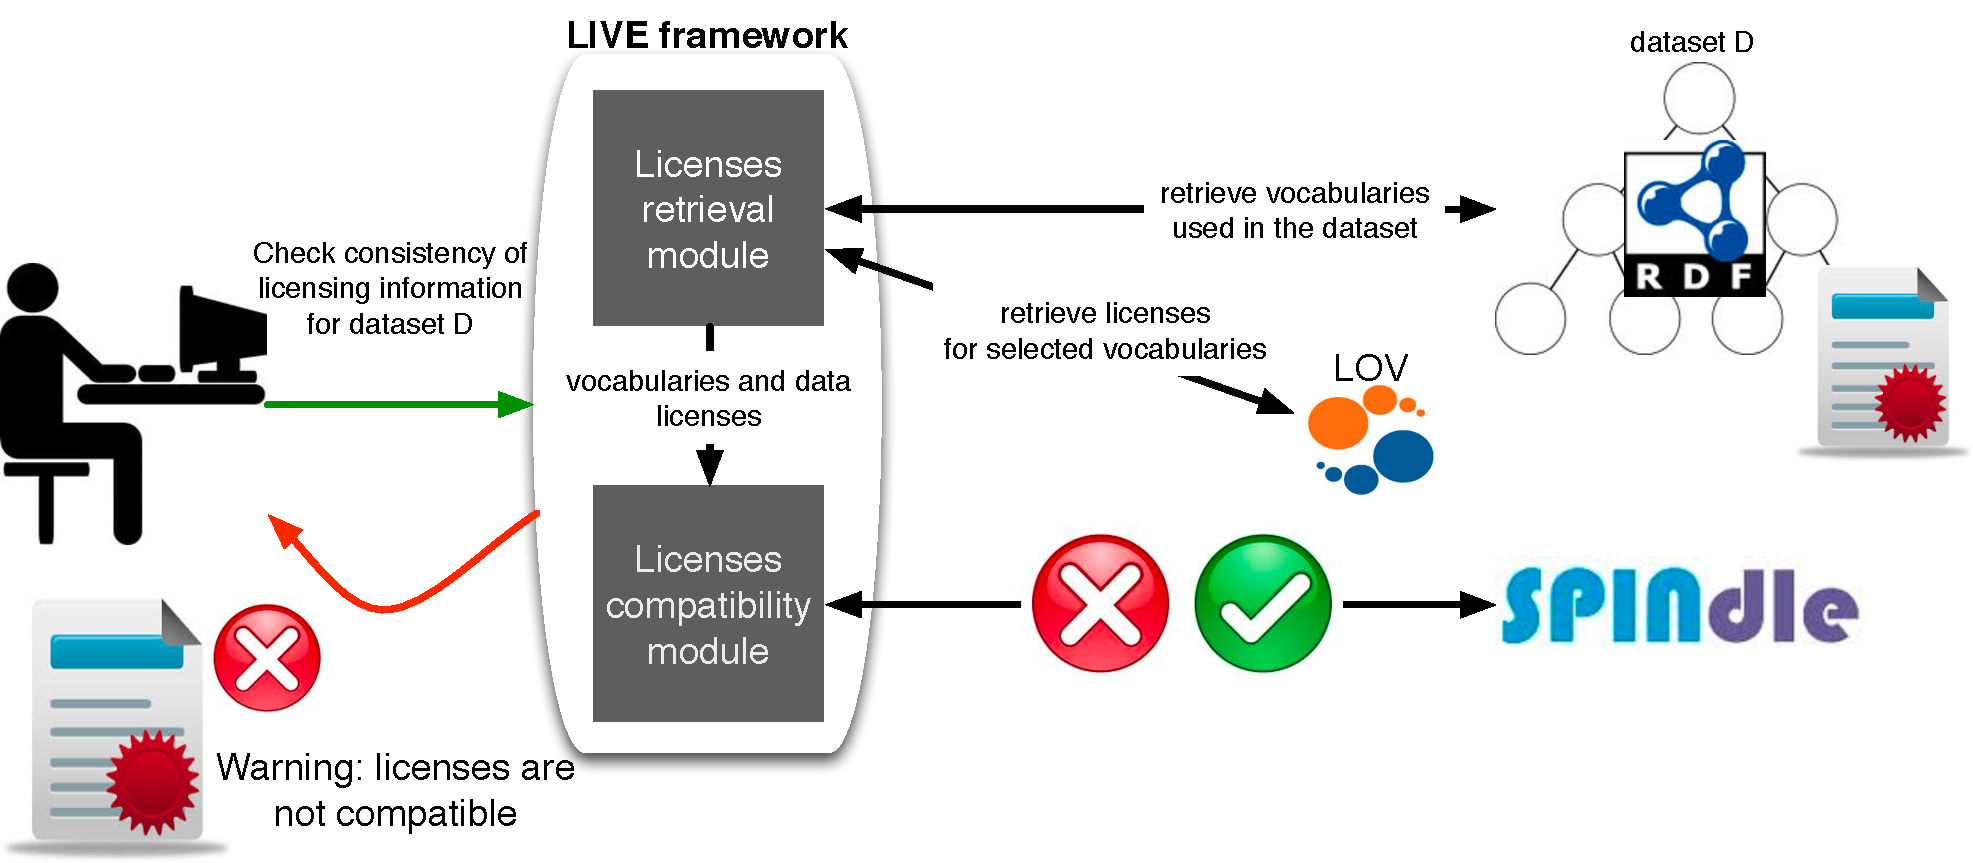
\includegraphics[width=12.0cm]{img/live-framework.pdf}
\caption{LIVE framework architecture.}
\label{fig:framework}
\end{figure}


\subsection{Licensing information from vocabularies and datasets.}
Two use-cases are taken into account: a SPARQL endpoint, or a VoID file in Turtle syntax. 
In the first use case, the tool retrieves the named graphs present in the repository, and then the user is asked to select the URI of the graph that needs to be checked. Having that information, a SPARQL query is triggered, looking for entities declared as \texttt{owl:Ontology}, \texttt{voaf:Vocabulary} or object  of the \texttt{void:vocabulary} property. The final step is to look up the LOV catalogue to check whether they declare any license. There are two options for checking the license: \textit{(i)} a \textit{``strict checking'' } where the \texttt{FILTER} clause contains exactly the namespace of the submitted vocabulary, or \textit{(ii)} a \textit{``domain checking''}, where only the domain of the vocabulary is used in the \texttt{FILTER} clause. This latter option is recommended in case only one vocabulary has to be checked for the license. 
%
In the second use case, the module parses a VoID file using a N3 parser for Javascript\footnote{\url{https://github.com/RubenVerborgh/N3.js}}, and then collects the declared vocabularies in the file, querying again LOV\footnote{Since LOV endpoint does not support the JSON format in the results, we have uploaded the data in \url{eventmedia.eurecom.fr/sparql}.} to check their licensing information. 
%
When the URIs of the licenses associated to the vocabularies and the dataset are retrieved, the module retrieves the machine-readable description of the licenses in the dataset of licenses~\cite{CabrioESWC2014}. More specifically, such dataset is composed by 37 licenses, comprising all the licenses adopted to certify data in the Linked Data cloud (as all the Creative Commons licenses\footnote{\url{http://creativecommons.org/licenses/}}), software licenses (as Mozilla Public License\footnote{\url{http://www.mozilla.org/MPL/2.0/}} and Microsoft License\footnote{\url{http://referencesource.microsoft.com/referencesourcelicensing.aspx}}), and additional licenses for other material on the Web (as the UK Open Government license, and the New Free Documentation License\footnote{\url{http://www.gnu.org/copyleft/fdl.html}}). The dataset provides the licenses in RDF using the Turtle syntax, however Creative Commons licenses are also available in XML/RDF format on the CC website\footnote{For instance, Creative Commons Attribution 4.0 license is available at \url{http://creativecommons.org/licenses/by/4.0/rdf}}.
Figure \ref{fig:livetoolUI} shows the user interface for quering a graph and sample results provided by LIVE tool.  

\begin{figure}[ht!b]
\centering{
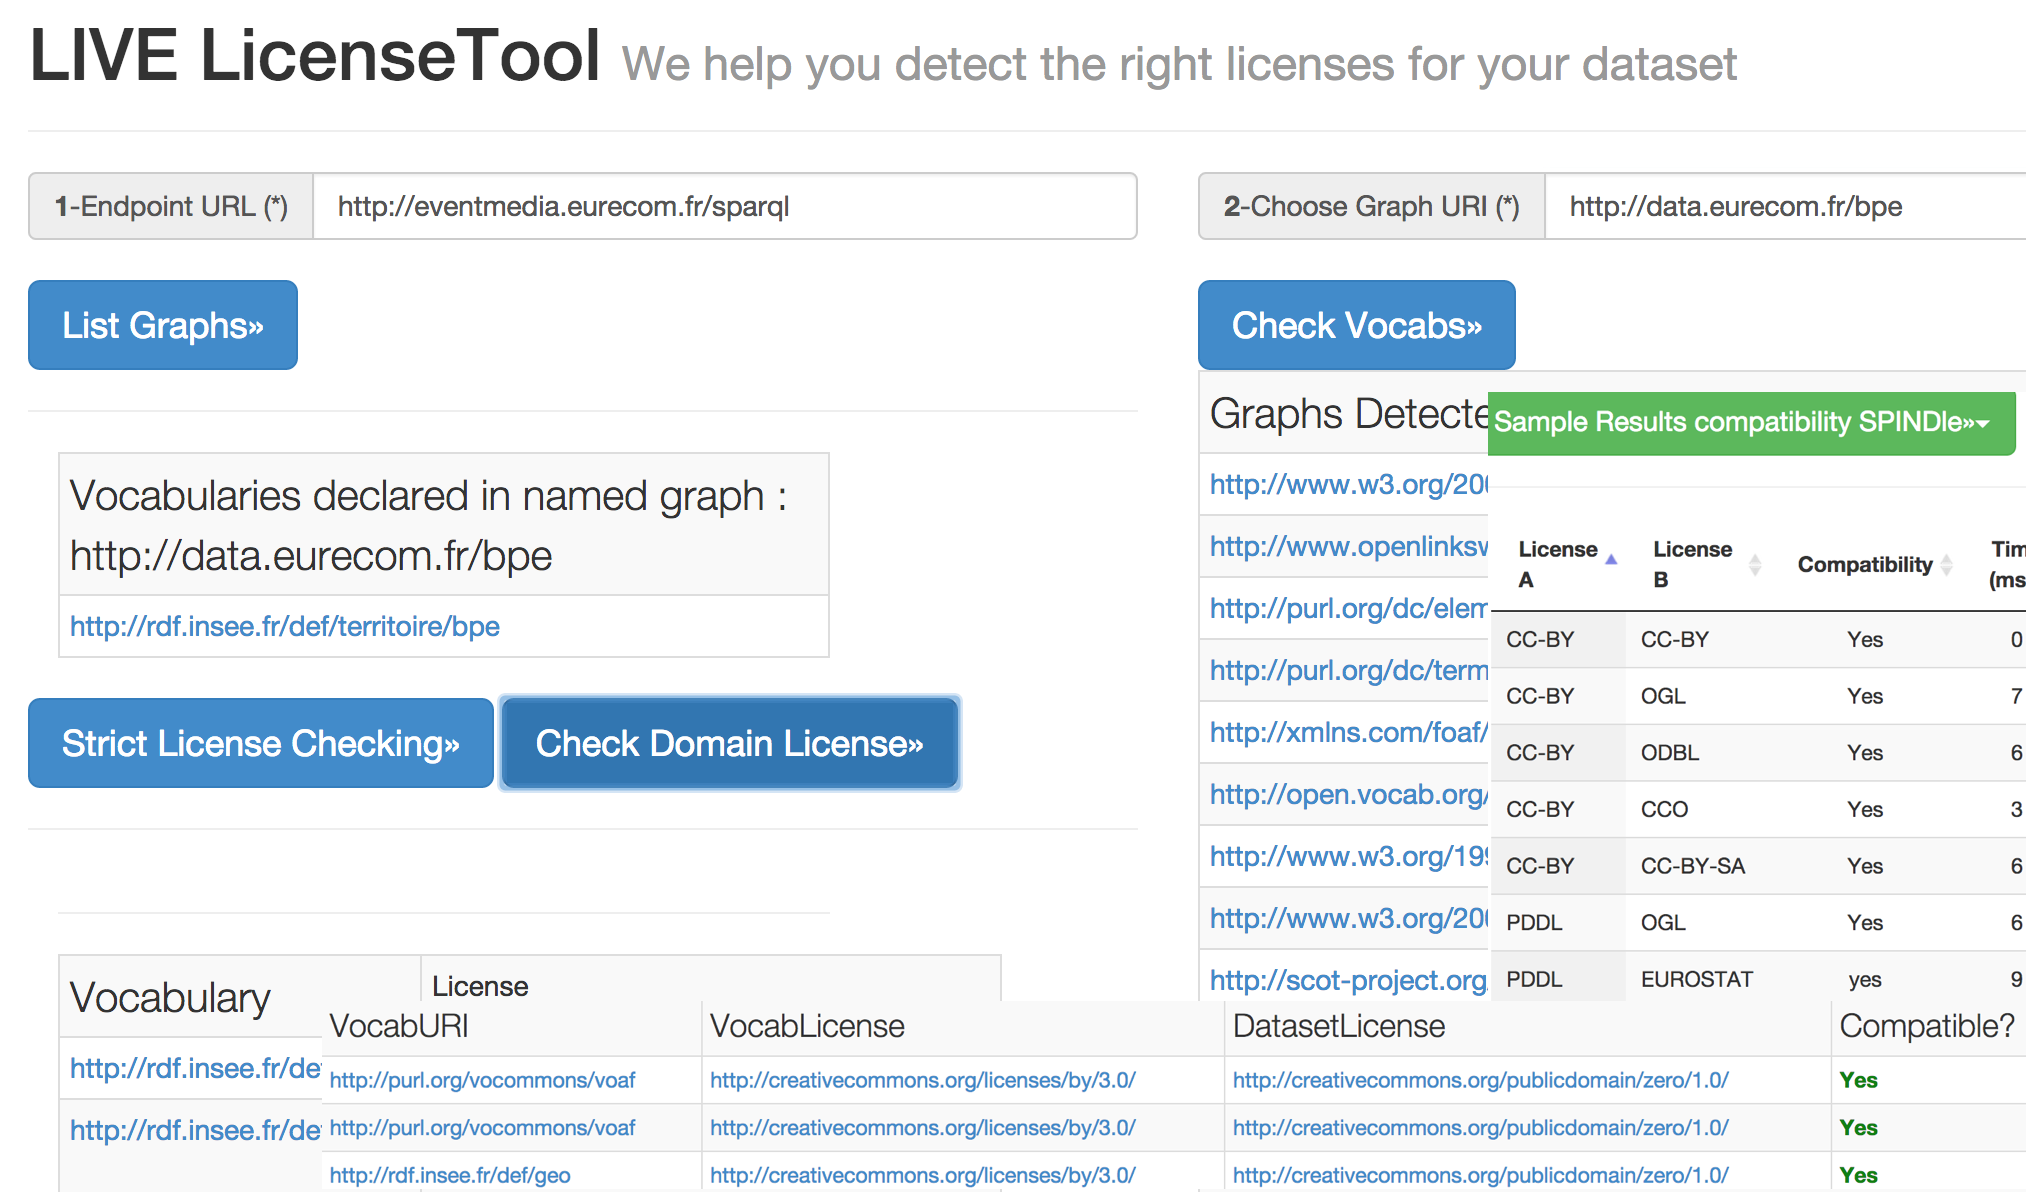
\includegraphics[scale=0.4]{img/LIVETool-UI.png}
\caption{LIVE tool user interface and sample results}
\label{fig:livetoolUI}
}
\end{figure}

\subsection{Licenses compatibility verification.}
The logic proposed in~\cite{DBLP:conf/semweb/GovernatoriRVG13} 
and the licenses compatibility verification process has been implemented using SPINdle~\cite{spindle} 
-- a defeasible logic reasoner capable of inferencing defeasible theories with hundredth of thousand rules.

%
\begin{figure}[ht!]
% \begin{wrapfigure}{r}{.5\textwidth}
\centering{
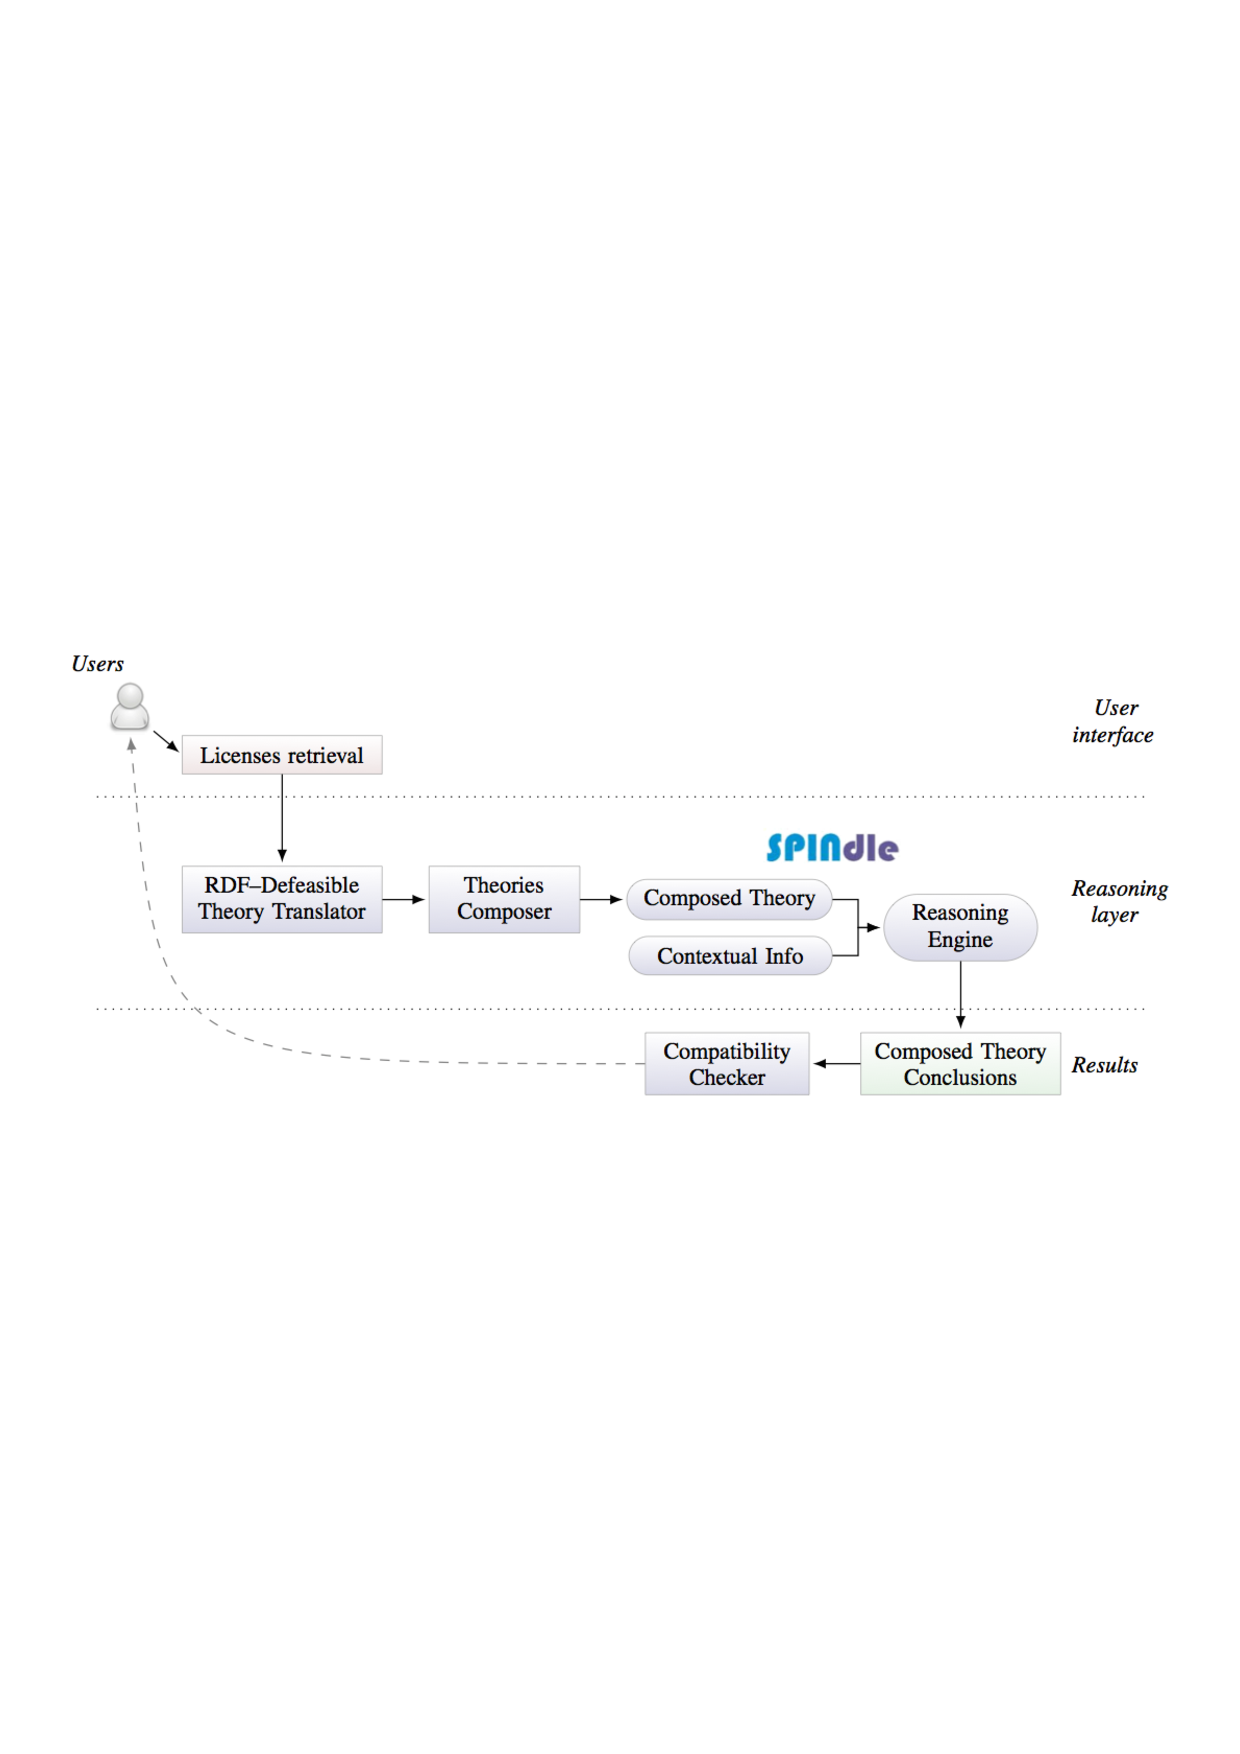
\includegraphics[scale=0.8]{img/composeTheories.pdf}
\caption{Licenses compatibility module.}
\label{figure:theoriesReasoningProcess}
}
\end{figure}
%

As depicted in Figure~\ref{figure:theoriesReasoningProcess},
after receiving queries from users,
the selected licenses (represented using RDF) will be translated into the DFL formalism supported by SPINdle using the \textit{RDF-Defeasible Theory Translator}. 
% If, 
% however,
% more than one license has been selected, % by user,
% then in order to verify the compatibility of different licensing terms, 
% the translated defeasible theories will first be composed into a single defeasible theory~\cite{DBLP:conf/semweb/GovernatoriRVG13} .
That is,
each RDF-triple will be translated into a defeasible rule based on the subsumption relation between the \textit{subject} and \textit{object} of a RDF-triples. In our case, we can use the subject and object of the RDF-triples as the antecedent and head of a defeasible rule, respectively. Besides, the translator also supports direct import from the Web and processing of RDF data into SPINdle theories. The \textit{RDF-Defeasible Theory Translator} will translate the RDF-licenses into the DFL formalism supported by SPINdle.

The translated defeasible theories will then be composed into a single defeasible theory based on the logic proposed in~\cite{DBLP:conf/semweb/GovernatoriRVG13},
using the \textit{Theories Composer}.
Afterwards,
the composed theory, 
together with other contextual information (as defined by user),
will be loaded into the SPINdle reasoner to perform a compatibility check before returning the results to the users.

We have evaluated the time performances of the LIVE framework in two steps (Table~\ref{tab:evalTool}).

\begin{table}[ht!]
\centering{

\begin{tabular}{|l|c|c|c|c|}
\specialrule{1pt}{1pt}{1pt}
 \textbf{Dataset} & \textbf{LicRe-} & \textbf{\#vocabu-} & \textbf{LicCompa-} & \textbf{LIVE(ms)}\\ 
 & \textbf{trieval(ms)} & \textbf{laries} & \textbf{tibility(ms)} & \\ \hline
  rkb-explorer-dblp & 4,499 &  1 & 0 & 4,499\\ \hline
  rkb-explorer-southampton & 14,693 & 1 & 0 & 14,693\\ \hline
  rkb-explorer-eprints & 3,220 & 1 & 0 & 3,220\\ \hline
  rkb-explorer-acm & 3,007 & 1 &  0 & 3,007\\ \hline
  rkb-explorer-wiki & 14,598 & 1 & 0& 14,598\\ \hline
  rkb-explorer-rae2001 & 3,343 & 1 &  0 & 3,343 \\ \hline
  rkb-explorer-citeseer & 2,760 & 1 & 0 & 2,760\\ \hline
  rkb-explorer-newcastle & 3,354 & 1 & 0 & 3,354\\ \hline
  rkb-explorer-kisti & 4,094 & 5 & 6 & 4,100\\ \hline
  270a.info & 13,202 & 48 & 8 & 13,210 \\ \hline
 
\end{tabular}\normalsize
\caption{Evaluation of the LIVE framework.}
\label{tab:evalTool}
}
\end{table}


First, we evaluate the time performances of the licenses compatibility module: it needs about 6ms to compute the compatibility of two licenses. Second, we evaluate time performances (Chrome v. 34) of the whole LIVE framework for the $10$ LOD datasets with the highest number of links towards other LOD datasets, considering both the licenses retrieval module and the licenses compatibility one. The results show that LIVE provides the compatibility evaluation in less than 5 seconds for $7$ of the selected datasets. Time performances of LIVE are mostly affected by the first module while the compatibility module does not produce a significant overhead. For instance, consider Linked Dataspaces\footnote{\url{http://270a.info/}}, a dataset where we retrieve the licensing information in both the dataset and the adopted vocabularies. In this case, LIVE retrieves in $13.20$s $48$ vocabularies, the license for the dataset is CC-BY, and the PDDL license is attached one of the vocabularies\footnote{\url{http://purl.org/linked-data/cube}}. The time for verifying the compatibility is $8$ms, leading to a total of $13.208$s.


\section{Summary and Perspectives}
\label{sec:summary-ch6}
In this chapter, we have presented an online tool to check the compatibility between datasets and vocabularies based on the RDF-defeasible of SPINdle. We have introduced the LIVE framework for licenses compatibility. The goal of the framework is to verify the compatibility of the licenses associated to the vocabularies exploited to create a RDF dataset and the license associated to the dataset itself. Several points have to be taken into account as future work. More precisely, in the present paper we consider vocabularies as data but this is not the only possible interpretation. For instance, we may see vocabularies as a kind of compiler, such that, after the creation of the dataset then the external vocabularies are no more used. In this case, what is a suitable way of defining a compatibility verification? We will investigate this issue as well as we will evaluate the usability of the online LIVE tool to subsequently improve the user interface

%our contributions on achieving some of the guidelines of the best practices of publishing Linked Data, by presenting the LOV catalogue, the harmonization of LOV with other catalogues, the importance of using semantics to rank vocabularies. Besides, we have presented Data2Ontology, a module aim at helping the reuse of existing vocabularies during the publication of data in Datalift. We finished by presenting \texttt{LIVE}, 